\chapter{Introduction}

Artificial intelligence (\acrshort{ai}) and, more specifically, \textbf{\acrlong{ml}} (\acrshort{ml}) has been through quite a journey since its inception in the 1940s and 1950s. From a small research domain, it has grown into a massive rapidly-developing field of research and applications with ramifications in many branches of science and technology. This growth is not surprising in a world where computers become more and more powerful and data, the bread-and-butter of machine learning, is becoming increasingly collectable, structured, available and queryable. Applications of \acrshort{ml} are as varied as they are numerous: spam filtering, fraud detection, face recognition, self-driving cars, robotics and automation, medical data analysis and diagnosis, simulation in particle physics... to name only a few. While it has already revolutionized many domains, \acrshort{ml} research has still a bright future ahead. In the last decade only, along with \textbf{\acrlong{dl}} (\acrshort{dl}), several new family of techniques have been (re-)discovered and have enabled unexpectedly-fast progress (\eg \acrlong{cnn}, \acrlong{gan}, transformers). One can only expect that the next ground-breaking \acrshort{ml} method is on the brink of being discovered in a research lab somewhere around the world. Aside from that, research is still ongoing of many fronts such as understanding, applying or improving existing methods.

Medicine is among the numerous fields where \acrshort{ml} is showing great promises. Although often misrepresented in the mainstream media as a tool that will eventually replace practitioners, the real potential of \acrshort{ml} in medicine actually lies in its capacity to become a strong, resilient and consistent assistant to the physicians \parencite{rajkomar2019machine} assisting them for tasks ranging from diagnosis and analysis to paperwork. Rather than replacing physicians, an \acrshort{ai}-based diagnosis system would be able to complement their opinion and advise them based on experiences of millions of other patients and colleagues. Moreover, such a system would be able to produce these advice based on a whole patient history and a very large number of parameters and sources of data that a human could not realistically consider (imaging, written reports, laboratory values, vital signs). However, the road to an \acrshort{ai}-assistant is still long and many questions and challenges have yet to be addressed. From a technological point of view, current research mostly focuses on improving solutions for tasks of significantly smaller scale and scope (\eg outlining organs in x-rays, detecting disease in \acrshort{ct}-scans, classifying skin cancer as malignant or benign \TODO{non imaging example}). Many recent contributions, although some arguably lacking scientific rigor, have claimed to have matched or surpassed human experts accuracies by applying \acrshort{ml} methods on different medical tasks \parencite{nagendran2020artificial}. Still, many challenges have yet to be solved. 

One of the major challenges faced when applying \acrshort{ml} to medical tasks is \textbf{data scarcity}. Not that data itself is lacking as \parencite{pramanik2019healthcare} reported that the amount of health data stored worldwide would reach 2,258 exabytes in 2020. What is scarce is actually data that is at least partially annotated and of good-enough quality to be used to train \acrshort{ml} models. Data scarcity has many causes: privacy concerns prevents sharing data, the annotation process is time-consuming and expensive, \acrshort{dl} methods are very data-hungry... 

This thesis focuses on the application of \acrlong{ml} to a field of medical imaging: \textbf{\acrlong{dp}} (\acrshort{dp}). \acrshort{dp} focuses on the analysis of large digitized glass slide images, also called \acrlong{wsi} (\acrshort{wsi}) containing tissue and cell samples. The particularity of a \acrshort{wsi} is its size as it can reach few billion pixels at minimum zoom level (see Figure \ref{fig:intro:wsi}). Glass slides screening have been part of clinical routine for some time now (\TODO{give an approximate date}) but digitization efforts have brought a bunch of new innovations allowing to analyse and share slides on a computer. It also opened the gates to automated analysis with \acrshort{ml} and \acrlong{dl} techniques.


\begin{figure}
  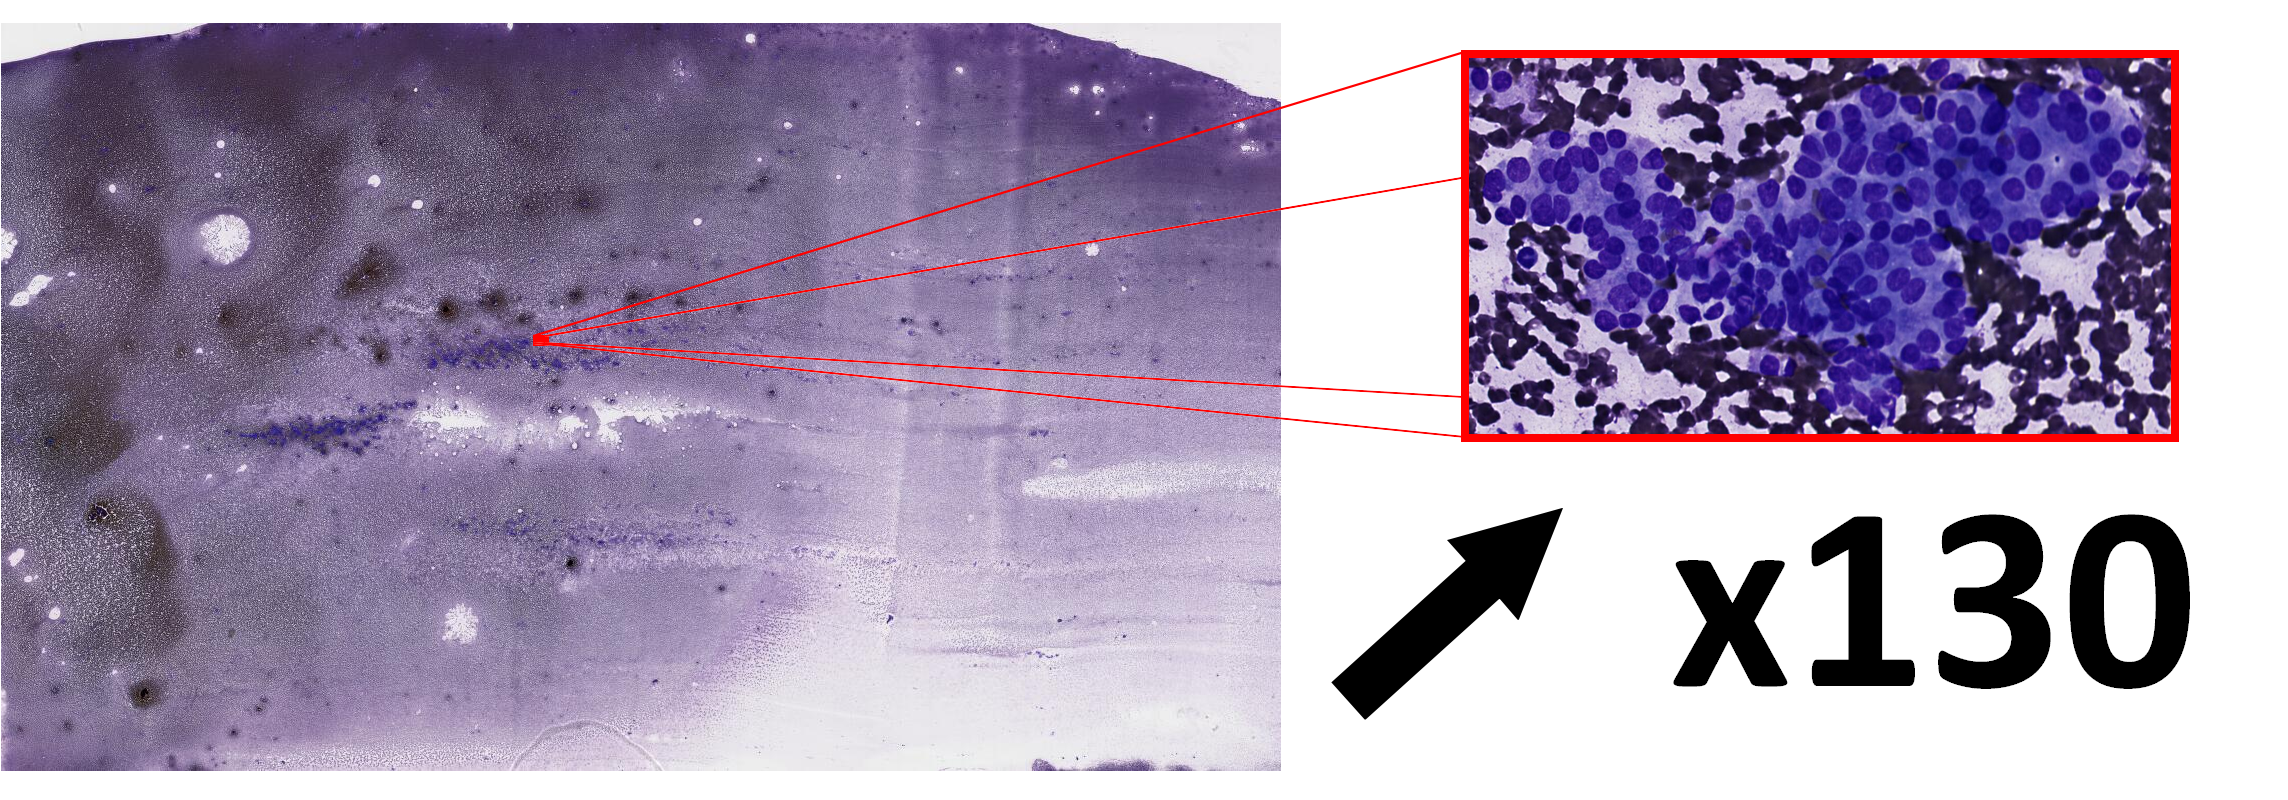
\includegraphics[scale=1]{intro/whole-slide-dim.png}
  \caption{A typical \acrlong{wsi} of size 163840 $\times$ 95744. To the left the original image, and to the right an structure of interest at zoom level $\times40$ from within the image (size: 1354 $x$ 736)}.
  \label{fig:intro:wsi}
\end{figure}

\section{Organization}

\section{Publications}

\begin{itemize}
  \item \fullcite{mormont2016sldc}
  \item \fullcite{mormont2018comparison}
  \item \fullcite{mormont2020multi}
  \item \fullcite{rubens2020biaflows}
\end{itemize}

